\chapter{Evaluation}
\label{sec:evaluation}

We evaluate our approach by implementing a number of dataflow kernels
for applications including advanced high-performance applications. We
measure productivity, in terms of lines of code, number of function
calls and cyclomatic complexity. We measure efficiency in terms of
performance and energy consumption and compare the software only
version, the version accelerated using MaxCompiler (manually written
dataflow kernels) and the proposed approach (MaxCompiler dataflow
kernels automatically generated using \fastc{}).

\label{sec:benchmark}

Our benchmark includes a variety of interesting real-life
applications, which are discussed in more detail in the remainder of
this chapter:
\begin{itemize}
\item \textbf{Numerical Differentiation} is a 1D stencil computation which
  is highly sensitive to floating point accuracy and tests the
  variable bit width optimisation capabilities of the proposed design
  flow. Numerical differentiation is used in situations where the
  analytical form of a functions is not available, for example on
  large sets of experimental data;
  \begin{comment}
  \item \textbf{Black Scholes Option Pricing} is a one dimensional
    stencil computation, with multiple time step iterations which
    requires the use of on-board DRAM to maximise efficiency; the Black
    Scholes model is one of the most commonly used models in finance for
    pricing derivatives of European options;
  \end{comment}
\item \textbf{Reverse Time Migration} is an advanced high-performance
  application for seismic imaging. It is the most widely used
  application in the Oil and Gas industry for identifying geological
  structures that resemble patches of oil. This application is also
  part of the HARNESS validation studies;
\item \textbf{Add Prediction} is an application for click-through rate
  prediction used in Microsoft's Bing search engine for Sponsored
  Search. This is an arithmetic intensive kernel, and requires the
  ability to effectively tune operator bit width and design parameters
  to reach reach timing closure. This is also part of the HARNESS
  validation studies;
\item \textbf{Bitonic Sorting Network} is a high-throughput sorting
  network for limited input size. It can be used as the first stage of
  a multi-gigabyte FPGA sorting algorithm, to separate the inputs into
  sorted buckets of up to 256 elements, after which a merging stage is
  applied. The sorting network is a recursively defined design, that
  heavily relies on compile-time loops, auxiliary function calls and
  input groups to generate a readable and parameterised
  description. Additionally by adapting operator bit-width to run-time
  inputs the network input width can be increased
  substantially,leading to improved throughput.
\end{itemize}

All dataflow designs are run on Maxeler MaxWorkstation
\cite{MaxWorkstation} which comprises:
\begin{itemize}
\item Vectis Dataflow Engine, 24 GB DRAM, Xilinx Virtex 6 FPGA Chip
\item Intel(R) Core(TM) i7 CPU 870 @ 2.93GHz, cache size 8192 KB
\item 16 GB DRAM connected to the CPU
\item DFEs connect to CPU via PCI Express gen2 x8
\end{itemize}

Theoretical memory bandwidth of the on-board DFE DRAM is 38 GB/s and
PCI-Express bandwidth (used for transferring data from the DRAM
connected to the CPU to the on-board DFE DRAM) is 2GB/s.

The process of placing and routing a dataflow design can take anywhere
from 20 minutes to several days. Since this is a stochastic process,
usually mutliple builds are started in parallel and when one
terminates successfully the whole build process is stop and that
design is used. Hence the build process requires substantial amount of
DRAM and CPU cores, particulary during the design space exploration
step where multiple instances of the same design are compiled to
identify maximum performance configuration. Hence the builds were ran
on the Custom Computing cluster machines:

\begin{itemize}
\item \texttt{cccad3} -- 2 8 core, hyperthreaded (16 threads) Intel
  Xeon E5-2650 CPUs at 2.00GHz, 20MB cache, 189 GB DRAM
\item \texttt{cccad2} -- 2 6 core, hyperthreaded (12 threads) Intel
  Xeon X5650 CPUs at 2.67GHz, 12 MB cache, 94 GB DRAM
\item \texttt{cccad1} -- 2 6 core, hyperthreaded (12 threads) Intel Xeon
  X5650 CPUs at 2.67GHz, 12 MB cache, 118 GB DRAM
\end{itemize}

All CPU applications are compiled using GCC 4.4 with all optimisations
enabled (-O3 flag) and FPGA Designs are compiled with MaxCompiler
2012.1.

\section{Numerical Differentiation}

Numerical differentiation is an important application in engineering
and can be used to estimate derivative values when an analytical form
of the function is not available. Consider for example the case of
measuring a sample of displacements form which we want to derive the
instantaneous speed. As explained in \Cref{sec:num-diff-back} a 5
point linear stencil can be used to approximate the value of the
derivative.

However, in practice, experimental data often contains noise (unwanted
random addition to a signal) which impacts the accuracy of the
estimation. To filter the noise, a smoothing step is applied to the
experimental data with the goal of improving the signal-to-noise
ratio. One of the most commonly used examples is the Savitzky-Golay
Filter \cite{savitzky1964smoothing} which applies a polynomial
regression to a set of a m data points, also a linear stencil
computation.  Using higher order stencils (up to a few hundreds even)
results in an smoother, less noisy regression.

Hence our implementation of the differentiation algorithm consists of
two steps: \emph{1)} applying the smoothing filter to the input data,
\emph{2)} estimating the derivative using a linear stencil. The
algorithm for an arbitrary stencil order is shown in Algorithm
\ref{alg:sg-numdiff}.

\begin{algorithm}
  \caption{Savitzky-Golay Numerical Differentiation}
  \label{alg:sg-numdiff}
  \begin{algorithmic}
    \Function{NumericalDifferentiation}{$values, Order, sCoefs, dCoefs, sn, dn, Step$}
    \State smoothValues $\gets$ \Call{Convolve}{$values, sCoefs, Order, sn$}
    \State diffValues  $\gets$ \Call{Convolve}{$values, dCoefs, Order, dn * step$}
    \State \Return $diffValues$
    \EndFunction

    \Function{Convolve}{$values, coeffs, Order, Normalizer$}
    \State result[] $\gets$ 0
    \For{$x = Order \to (nCoefs - Order)$}
    \For{$c = 1 \to nCoefs$}
    \State result[x] $\gets$ result[x] + value[x - Order + c] * coeffs[c]
    \EndFor
    \State result[x] $\gets$ result[x] / Normalizer
    \EndFor
    \State \Return result
    \EndFunction
  \end{algorithmic}
\end{algorithm}

Our \FAST{} dataflow designs consist of two kernels one for smoothing
and one for differentiation. We explore the possibility of generating
an efficient run-time reconfigurable design either for improving
design performance, or for supporting larger dimension stencils, via
time-sharing. We measure resource usage and performance for stencil
size of 5, 7 and 9 points and estimate the resource usage for larger
stencils to identify sizes at which run-time reconfiguration becomes
convenient. To maximise performance we write a parametrised design
which can be parallelised up to the point where it becomes memory
bound.

Since the design uses PCI-E the maximum parallelism that can be
achieved before it becomes I/O bound is given by:
$$\frac{\text{PCI-E bits per cycle}}{\text{kernel input bits}} = \frac{128}{32} = 4$$

Hence, when using PCI-E a kernel replication factor of 4 is ideal for
maximising throughput.

If data were available straight from FPGA DRAM the design parallelism
could be increased to:
$$\frac{\text{memory bits per cycle}}{\text{kernel input bits}} = \frac{1536}{32} = 48$$

However, for this algorithm transferring data to on-board DRAM will
not improve overall throughput since data are only used once, hence we
investigate the PCI-E design.

The measured resource usage scales linearly with the parallelism level
as shown in \Cref{table:nd1} and shows that for a 7 point stencil,
approximately 10 pipelines can mapped onto the FPGA. However, beyond
80\% resource usage level, the design usually becomes fairly congested
and fails to route or takes an extremely large time to achieve timing
closure.

\begin{table}[ht!]
  \begin{tabularx}{\textwidth}{X|X|X|X|X}
    Pipes & LUT Usage & FF Usage & DSP Usage & BRAM Usage \\
    \hline\hline
    1     & 10.01     & 6.65     & 8.45      & 0.75       \\
    2     & 18.91     & 13.21    & 17.51     & 1.50       \\
    4     & 37.13     & 25.32    & 33.12     & 3.75       \\
    6     & 56.17     & 39.28    & 50.31     & 4.50       \\
    8     & 79.63     & 51.22    & 49.55     & 7.75       \\
  \end{tabularx}
  \caption{Pipeline scalability of the numerical differentiation algorithm for a 7 point stencil.}
  \label{table:nd1}
\end{table}

\Cref{table:nd2} shows that the maximum achievable stencil width with
the static design (which uses both kernels onto the FPGA chip) is 29
whereas using run-time reconfiguration to swap the individual kernels
increases the maximum stencil width to around 59 points (computed an
assumed 4 parallel pipelines as shown on lines 4, 8 and 9 of
\Cref{table:nd2}).

\begin{table}[ht!]
  \begin{tabularx}{\textwidth}{X|X|X|X|X|X}
    Kernel                    & Stencil Width & LUT Usage & FF Usage & DSP Usage & BRAM Usage   \\
    \hline\hline
    \multirow{4}{*}{GSDiff}   & 5             & 2.03      & 1.55     & 0.99      & 0            \\
    & 7             & 2.79      & 2.08     & 2.92      &              \\
    & 9             & 3.33      & 2.48     & 3.76      & 0            \\
    \cline{2-6}
    & \multicolumn{5}{c}{Max = $100 / 3.76 * 9 / 4 = 239 / 4 = 59 $} \\
    \hline
    \multirow{4}{*}{GSSmooth} & 5             & 2.34      & 1.44     & 2.23      & 0            \\
    & 7             & 2.91      & 1.81     & 2.97      & 0            \\
    & 9             & 3.47      & 2.21     & 3.91      & 0            \\
    \cline{2-6}
    & \multicolumn{5}{c}{Max = $100 / 3.91 * 9 / 4 = 239 / 4 = 57 $} \\
    \hline
    Both                       & \multicolumn{5}{c}{Max = $100 / (3.91 + 3.76) * 9 / 4 = 29 $}  \\
  \end{tabularx}
  \caption{Resource usage per stencil width, per kernel, per compute pipe.}
  \label{table:nd2}
\end{table}


The \FAST{} dataflow kernel that implements the differentiation
operation is shown in Listing {}. It uses no API (non-user defined)
function calls and a total of 20 lines of code, compared to the
original MaxCompiler design which requires 14 API calls and 37 lines
of code.


% \section{Black Scholes}nn

\section{Reverse Time Migration}
\label{sec:RTM}
The Reverse Time Migration method for seismic imaging which is used to
detect geological structures, based on the Earth's response to
injected acoustic waves. Background on istropoic acoustic modelling
and the RTM algorithm is introduced in \Cref{sec:rtm-back}. For the
purpose of our implementation we approximate the differential equation
using stencil computation to perform a fifth-order Taylor expansion in
space and first-order expansion in time.

We use \FAST{} to implement the dataflow kernels for both read and
write memory controllers (\texttt{kernel\_CmdRead},
\texttt{kernel\_CmdWrite}) and the application compute kernel
(\texttt{kernel\_RTM}).  To illustrate the benefits of our approach we
analyse the results of using the debugging aspect of
\Cref{sect:asp_debug}. \Cref{table:loc} compares the number of lines
of code required for the \FAST{} with aspect design with the
equivalent MaxCompiler implementation showing a reduction in code size
of up to 42\% for the run-time reconfigurable design and a reduction
in the number of API calls (including debug calls) of up to 67\% which
translate to increased productivity.

\begin{table}[!h]

  \centering
  \begin{tabular}{c|ccc|cc}
    \hline
    \multirow{2}{*}{\bf{Kernel}} & \bf{Aspect } & \multicolumn{2}{c|}{\bf{\FAST{}}} & \multicolumn{2}{c}{\bf{MaxCompiler}}                   \\
    \                            & \bf{LOC}     & \bf{LOC}                       & \bf{\# API calls} & \bf{LOC} & \bf{\#API Calls} \\
    \hline \hline
    CmdRead                      & 12           & 26                             &      6         & 59       &      39        \\
    CmdWrite                     & 12           & 28                             &      39        & 79      &       56         \\
    RTM Static                   & 12           & 246                            &     43         & 403     &       175        \\
    RTM RTR                      & 12           & 377                            &     91         & 669     &       275       \\
  \end{tabular}
  \caption{Code measures for the RTM kernels comparing \FAST{} and
    MaxCompiler.}
  \label{table:loc}
\end{table}

Results of the design space exploration using the aspect in
\Cref{fig:aspect-exploration} with variable mantissa illustrate
the trade-offs between accuracy and resource usage
(\Cref{fig:precision}). We observe irregular, large variations
when decreasing the mantissa from 18 to 16 and 24 to 22 which is the
effect of the backend tools mapping arithmetic to a combination of
both DSPs and LUT/FF elements. The mantissa boundaries at which this
optimisation occurs are platform specific, depending on the
architecture of the DSPs. Hence, automating this optimisation via
aspects and decoupling it from the original source code makes the
application more portable and facilitates discovery of interesting
trade-off opportunities using design space exploration.

\begin{figure}[!h]
  \centering
  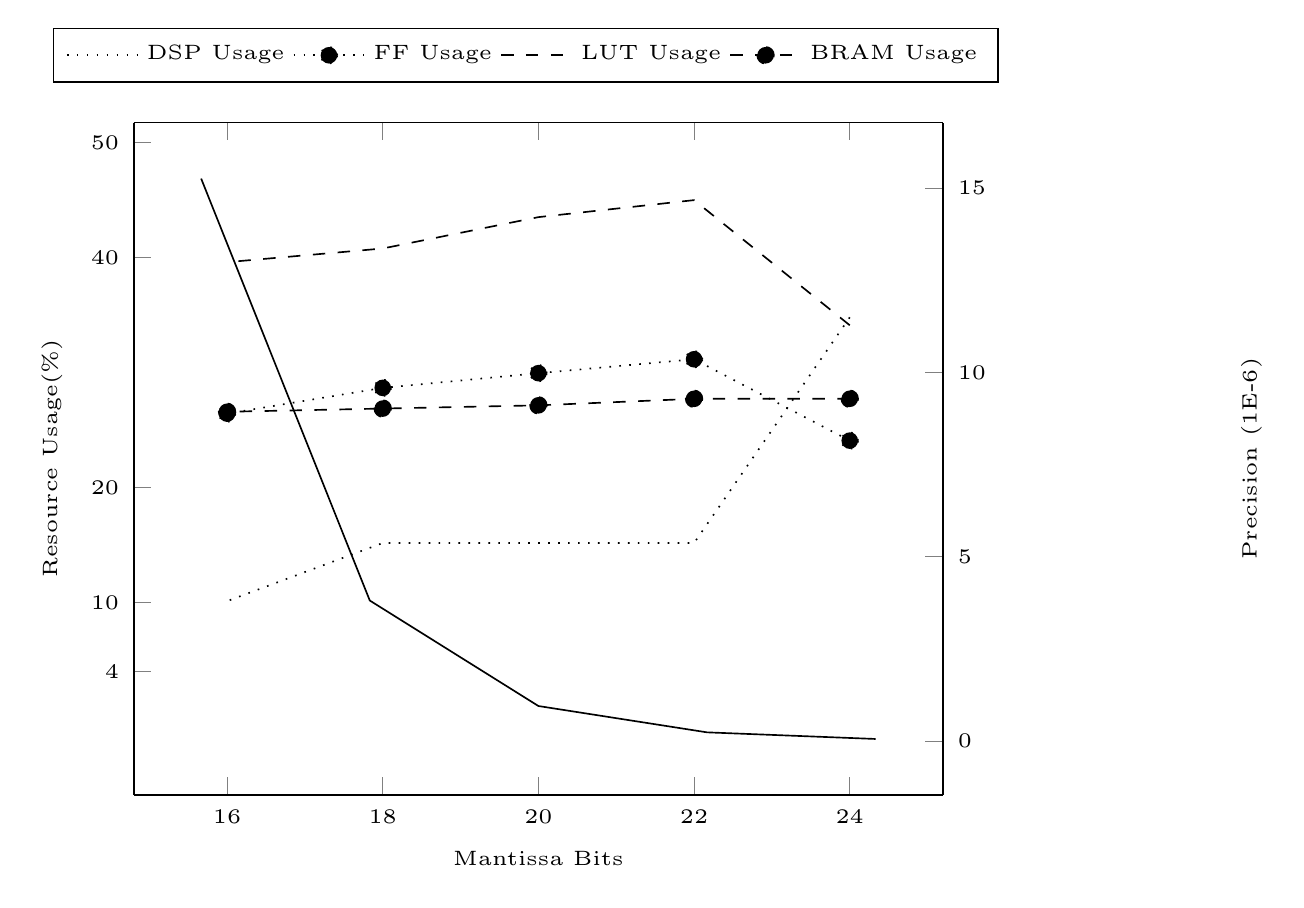
\begin{tikzpicture}[scale=1.5]
    \selectcolormodel{gray}
    \begin{axis}[
      xmin=16,
      ymin=0,
      % no markers,
      enlargelimits=0.15,
      font=\tiny,
      axis y line*=left,
      xlabel=Mantissa Bits,
      ylabel=Resource Usage(\%),
      xtick={16,18,20,22,24},
      ytick={4, 10, 20, 40, 50, 70, 80, 100},
      legend columns=4,
      legend entries={
        DSP Usage,
        FF Usage,
        LUT Usage,
        BRAM Usage},
      legend style={
        at={(-0.1,1.1)},
        anchor=west
      }
      ]
      \addplot[dotted] coordinates {
        (24, 34.82)
        (22, 15.18)
        (20, 15.18)
        (18, 15.18)
        (16, 10.12)
      };
      \addplot[mark=*, dotted] coordinates {
        (24, 24.09)
        (22, 31.17)
        (20, 29.96)
        (18, 28.68)
        (16, 26.44)
      };
      \addplot[mark=none, dashed] coordinates {
        (24, 34.13)
        (22, 45.02)
        (20, 43.54)
        (18, 40.81)
        (16, 39.62)
      };
      \addplot[mark=*, dashed] coordinates {
        (24, 27.73)
        (22, 27.73)
        (20, 27.16)
        (18, 26.88)
        (16, 26.60)
      };
    \end{axis}
    \begin{axis}[
      ylabel=Precision (1E-6),
      font=\tiny,
      axis y line*=right,
      axis x line=none,
      ylabel style={at={(1.35,0.5)}}
      ]
      \addplot[mark=none] coordinates {
        (16, 15.2585)
        (18, 3.8146)
        (20, 0.9536)
        (22, 0.2394)
        (24, 0.0596)
      };
    \end{axis}
  \end{tikzpicture}
  \caption{Exploration of accuracy vs resource usage trade-offs using
    the aspect shown in \Cref{fig:aspect-exploration} with variable
    mantissa.}
  \label{fig:precision}
\end{figure}

Computation precision using floating point types can be estimated by:
$$ \text{precision} = \frac{1}{2^{\text{mantissa bits}}} $$

\begin{table}[!ht]
  \begin{tabularx}{\textwidth}{c|c|X|X|X|X|X}
    Exp. & Mant. & FF    & BRAM  & LUT   & DSP   & Precision ($1E-6$) \\
    \hline\hline
    8      & 24    & 24.09 & 27.73 & 34.13 & 34.82 & 0.0596             \\
    8      & 22    & 31.17 & 27.73 & 45.02 & 15.18 & 0.2384             \\
    8      & 20    & 29.96 & 27.16 & 43.54 & 15.18 & 0.9536             \\
    8      & 18    & 28.68 & 26.88 & 40.81 & 15.18 & 3.8146             \\
    8      & 16    & 26.44 & 26.60 & 39.62 & 10.12 & 15.2585            \\
  \end{tabularx}
  \caption{Resource usage vs accuracy trade-off exploration data.}
\end{table}

The DSP balancing aspect shown in Fig.~\ref{fig:aspect-DSP} allows to
explore the resource trade-offs of implementing arithmetic operations
in either DSPs or LUTs and FFs (Fig.~\ref{fig:arith}) and helps to
avoid over mapping on DSPs for arithmetic intensive applications.

\begin{figure}[!h]
  \centering
  \hspace{-2cm}
  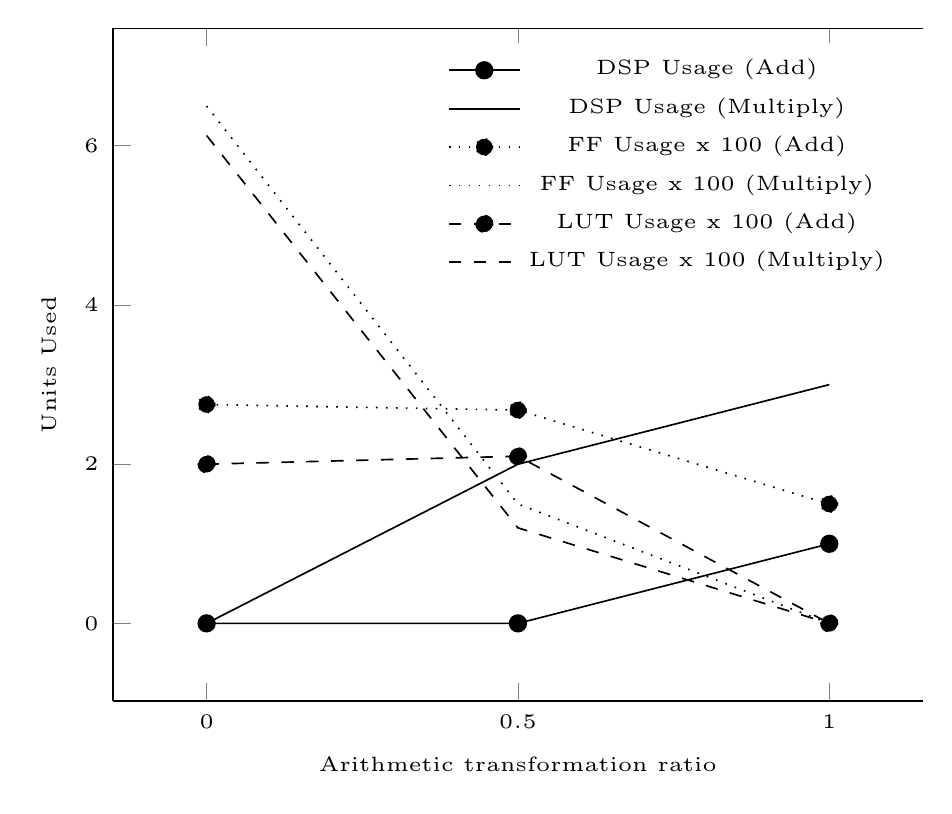
\begin{tikzpicture}[scale=1.5]
    \selectcolormodel{gray}
    \begin{axis}[
      xmin=0,
      ymin=0,
      % no markers,
      enlargelimits=0.15,
      font=\tiny,
      axis y line*=left,
      xlabel=Arithmetic transformation ratio,
      ylabel=Units Used,
      xtick={0, 0.5, 1},
      legend columns=1,
      legend entries={
        DSP Usage (Add),
        DSP Usage (Multiply),
        FF Usage x 100 (Add),
        FF Usage x 100 (Multiply),
        LUT Usage x 100 (Add),
        LUT Usage x 100 (Multiply),
      },
      legend style={
        draw=none
      }
      ]
      \addplot[mark=*] coordinates {
        (0, 0)
        (0.5, 0)
        (1, 1)
      };
      \addplot[] coordinates {
        (0, 0)
        (0.5, 2)
        (1, 3)
      };
      \addplot[mark=*, dotted] coordinates {
        (0, 2.75)
        (0.5, 2.68)
        (1, 1.50)
      };
     \addplot[dotted] coordinates {
        (0, 6.5)
        (0.5, 1.5)
        (1, 0)
      };
      \addplot[mark=*, dashed] coordinates {
        (0, 2)
        (0.5, 2.1)
        (1, 0)
      };
      \addplot[dashed] coordinates {
        (0, 6.13)
        (0.5, 1.2)
        (1, 0)
      };
    \end{axis}
  \end{tikzpicture}
  \caption{Exploration of DSP and LUT/FF balancing for functional units
    implementing a single arithmetic operation using the aspect shown
    in Fig.~\ref{fig:aspect-DSP}.}
  \label{fig:arith}
\end{figure}

Design space exploration using the aspect in
Fig.~\ref{fig:aspect-exploration} with increasing parallelism level
can be used to investigate design scalability. For example, for the
described RTM implementation, Fig.~\ref{fig:scalability} shows that
performance scales linearly with the number of parallel pipelines and
that significant speedups can be obtained by the \FAST{} dataflow
design compared to the CPU only implementation. Depending on the
problem size, our approach can be used to achieve a significant
speedup over software only versions which is comparable with the best
published FPGA results for static designs
\cite{Xinyu:Qiwei:Luk:Qiang:Pell:2012}, \cite{araya2011assessing}.


\begin{figure}[!h]
  \centering
  \hspace{-1cm}
  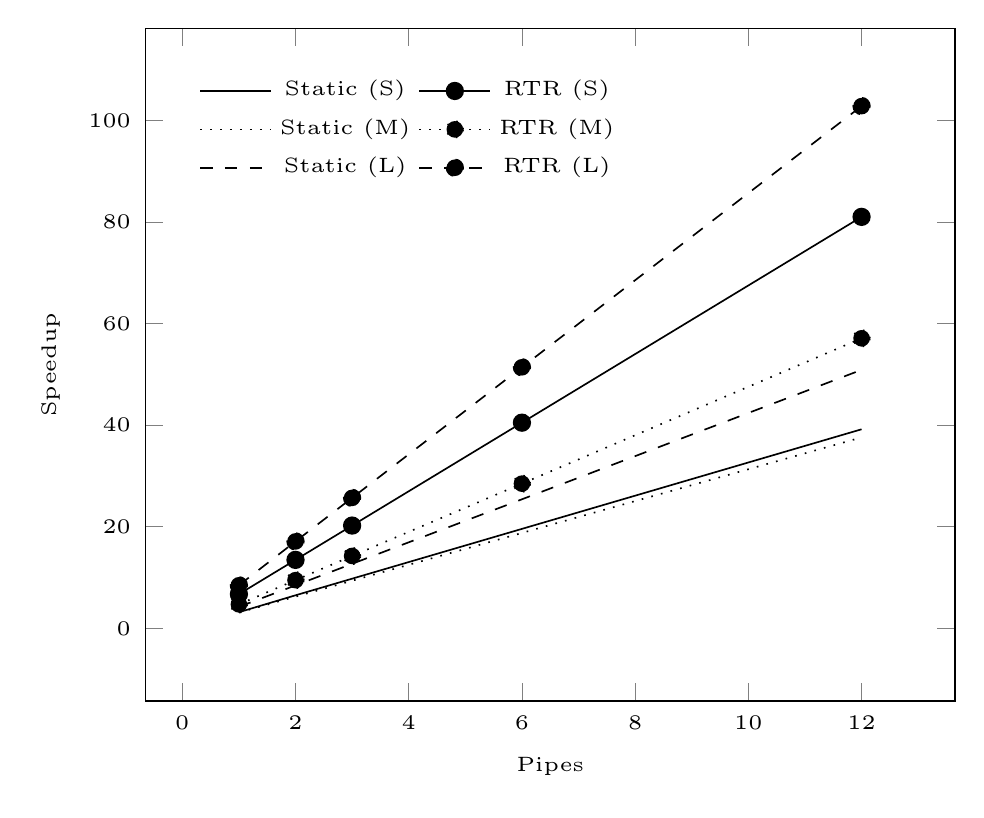
\begin{tikzpicture}[scale=1.5]
    \begin{axis}[
      xmin=1,
      ymin=1,
      enlargelimits=0.15,
      % no markers,
      font=\tiny,
      xlabel=Pipes,
      ylabel=Speedup,
%      xtick={1,2,3,6,12},
%      ytick={4, 10, 20, 40, 50, 70, 80, 100},
      legend columns=2,
      legend entries={
        Static (S),
        RTR (S),
        Static (M),
        RTR (M),
        Static (L),
        RTR (L)},
      legend style={
        draw=none,
        at={(0.05,0.85) },
        anchor=west
      }
      ]
      \addplot[mark=none] coordinates {
        (1, 3.2)
        (2, 6.53)
        (3, 9.8)
        (6, 19.6)
        (12, 39.2)
      };
      \addplot[mark=*] coordinates {
        (1, 6.75)
        (2, 13.5)
        (3, 20.25)
        (6, 40.5)
        (12, 81)
      };
      \addplot[dotted] coordinates {
        (1, 3.13)
        (2, 6.26)
        (3, 9.4)
        (6, 18.8)
        (12, 37.6)
      };
      \addplot[mark=*, dotted] coordinates {
        (1, 4.75)
        (2, 9.51)
        (3, 14.27)
        (6, 28.5)
        (12, 57.1)
      };
      \addplot[mark=none, dashed] coordinates {
        (1, 4.25)
        (2, 8.48)
        (3, 12.725)
        (6, 25.42)
        (12, 50.9)
      };
      \addplot[mark=*, dashed] coordinates {
        (1, 8.5)
        (2, 17.13)
        (3, 25.7)
        (6, 51.4)
        (12, 102.8)
      };
    \end{axis}
  \end{tikzpicture}
  \caption{Scalability of the RTM dataflow design explored using the aspect
    shown in Fig.~\ref{fig:aspect-exploration}.}
  \label{fig:scalability}
\end{figure}




Fig.~\ref{fig:scalability} also shows a model of the performance
benefits of using a run-time reconfigurable implementation generated
using the proposed aspect-oriented approach. Two configurations were
created for the RTM \FAST{} kernel. Since, in our model, during the
first half of the execution time, the backward propagation and imaging
functions are idle, the first configuration requires only half the
resources. Hence, the number of parallel pipelines can be doubled,
halving the execution time of the first configuration. The speedup
obtained is comparable to \cite{Xinyu:Qiwei:Luk:Qiang:Pell:2012}, but
the partitioning and optimisation exploration process is automated via
aspects, which increases developer productivity. The automated process
improves portability of the design, allowing optimisations based on
design space exploration to be carried out on various platforms (hence
subject to varying resource constraints) without manual intervention.




\section{Bitonic Sort}

Sorting networks \cite{batcher1968sorting} are an interesting
benchmark application for our approach since it is both an important
application but also fairly challenging to fit into the proposed
programming model:
\begin{itemize}
\item Sorting networks constitute the basic blocks for
  high-performance multi-gigabyte sorting which in the context of the
  HARNESS project, is an important case study for key cloud
  applications;
\item Sorting networks are not easily mapped to FPGA since resource
  constraints limited considerably the input size of the network; for
  example, our sorting network implementation fails to achieve timing
  closure
\item Comparison based sorting requires very little arithmetic, which
  is a major disadvantage on the Maxeler Platform, since DSPs cannot
  be utilised
\item Sorting in general is an application that does not map well onto
  the streaming model of computation, since due to the aforementioned
  resource constraints, merging of buckets of values is required which
  leads to a feed-back loop in the design;
\end{itemize}

We implement a bitonic sorting network for inputs of $n$ arrays of
size $k = (4, 8, 32, 64, 128, 256)$ elements. We compare the
performance of the design with the ANSI C implementation of
\texttt{qsort()}
\footnote{http://www.umcs.maine.edu/~chaw/200801/capstone/n/qsort.c}
which is a hybrid of insertion-sort and quicksort. For a fixed network
size, we vary the input size to compare the software and hardware
implementations and report the average results of 50 runs.

The implemented sorting network has the following properties:
\begin{itemize}
\item $\text{complexity} = \text{network depth} = \frac{n * log(n)}{2} = O(log^2(n))  $
\item $\text{comparators} = n * log(n) * (log(n) + 1) / 4 = O(n * log^2(n)) $
\end{itemize}


Execution results ares summarised in and include in show that the hardware version
outperforms the software version for values of n larger than $2^4$
with speedups increasing from 1.25X to 24X, in proportion with the
value of n.  Also the execution time is dominated by data transfer
time over PCIe from main memory to the FPGA accelerator. The impact of
the pipeline stages is so small that it cannot be measured accurately
using the Linux timing utilities (e.g. \texttt{gettimeofday()}).

Given that execution time is dominated by the transfer time,
reconfiguring the design to increase parallelism will bring a small
performance benefit.  The situation changes when the network is used
as part of a general purpose sorting algorithm. The complexity $( O(N/k
* logn * log(n/k)) $ decreases linearly with the increase in the network
width. This would provide the motivation to adapt the network to input
patterns, switching to larger networks for small observed values.

Hence it is only necessary to reconfigure when a change in the input
pattern is detected that requires us to use a different
precision. (e.g. floating point vs int).

One factor to consider is that, reducing to smaller network sizes can
also decrease the communication overhead. Since all network inputs
must be present, additional padding is required for arrays that are
not of a length which is a power of two. (Requires additional data)

Results of varying the word length show that decreasing word width and
varying the type (floating or fixed point, based on the input
characteristics) allow us to build larger network sizes. This can more
than double the performance of networks for small input values.

\begin{table}[!ht]
  \begin{tabularx}{\textwidth}{X | X | X | X | X | X}
    \hline
    Type & Width & Max. Network Size & Resource Usage (LUT/FF) & Overmaps At Next Size & Meets Timing at Next Size \\
    \hline
    \hline
    int & 32 & 128 & 127344 / 260434 & yes & no \\
    \hline
    int & 16 & 128 & 127344 / 260434 & no (23343 / 343332) & no \\
    \hline
    int & 8 & 256 & 95430 / 188245 & no (260878 / 458532) & no \\
    \hline
    float & (8, 24) & 64 & 101758 / 107901 & yes & no \\
    \hline
    fixed point & (8, 24) & 128 & 127344 / 260434 & yes & no \\
    \hline
    fixed point & (24, 8) & 128 & 127344 / 260434 & yes & no \\
  \end{tabularx}
  \caption{Results of exploring different network sizes and data types for the bitonic sorting network}
\end{table}




\begin{comment}
  \begin{figure}[!h]
    \centering
    \vspace{0.35cm}
    \hspace{-8mm}
    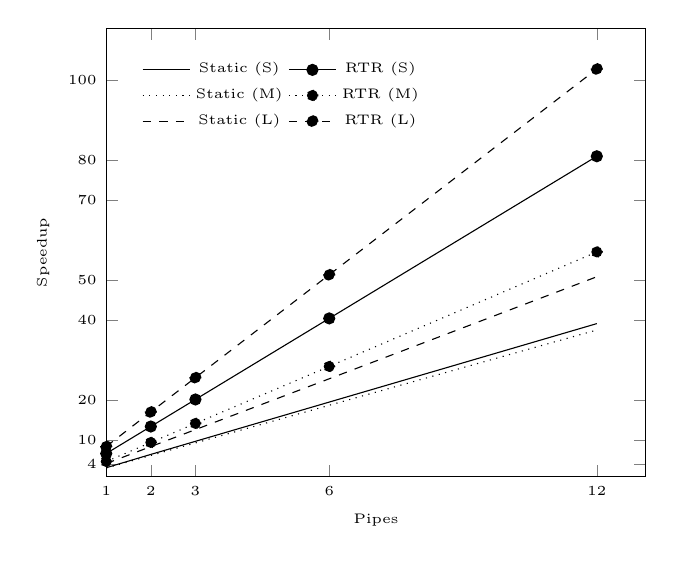
\begin{tikzpicture}[scale=1]
      \selectcolormodel{gray}
      \begin{axis}[
        xmin=1,
        ymin=1,
        % no markers,
        font=\tiny,
        xlabel=Pipes,
        ylabel=Speedup,
        xtick={1,2,3,6,12},
        ytick={4, 10, 20, 40, 50, 70, 80, 100},
        legend columns=2,
        legend entries={
          Static (S),
          RTR (S),
          Static (M),
          RTR (M),
          Static (L),
          RTR (L)},
        legend style={
          draw=none,
          at={(0.05,0.85) },
          anchor=west
        }
        ]

        \addplot[mark=none] coordinates {
          (1, 3.2)
          (2, 6.53)
          (3, 9.8)
          (6, 19.6)
          (12, 39.2)
        };
        \addplot[mark=*] coordinates {
          (1, 6.75)
          (2, 13.5)
          (3, 20.25)
          (6, 40.5)
          (12, 81)
        };
        \addplot[dotted] coordinates {
          (1, 3.13)
          (2, 6.26)
          (3, 9.4)
          (6, 18.8)
          (12, 37.6)
        };
        \addplot[mark=*, dotted] coordinates {
          (1, 4.75)
          (2, 9.51)
          (3, 14.27)
          (6, 28.5)
          (12, 57.1)
        };
        \addplot[mark=none, dashed] coordinates {
          (1, 4.25)
          (2, 8.48)
          (3, 12.725)
          (6, 25.42)
          (12, 50.9)
        };
        \addplot[mark=*, dashed] coordinates {
          (1, 8.5)
          (2, 17.13)
          (3, 25.7)
          (6, 51.4)
          (12, 102.8)
        };
      \end{axis}
    \end{tikzpicture}
    \caption{Scalability of the RTM dataflow design explored using the aspect
      shown in Fig.~\ref{fig:aspect-exploration}.}
    \label{fig:scalability}
  \end{figure}
\end{comment}
